\documentclass{standalone}
%\usepackage{pgfplots}
\usepackage{tikz}

\title{Hutton's formula}
\begin{document}
	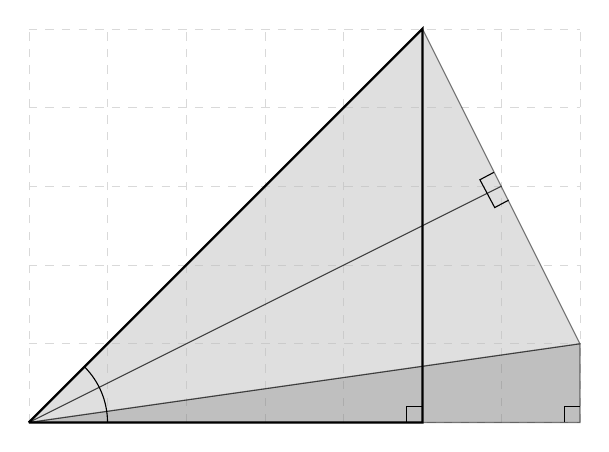
\begin{tikzpicture}
		\draw[help lines, color=gray!30, dashed] (0,0) grid (7,5);
		\draw[-,fill=gray, opacity=0.5] (0,0) -- (7,0) -- (7,1) -- (0,0);
		\draw[-,fill=gray!50!white, opacity=0.5] (0,0) -- (7,1) -- (6,3) -- (0,0);
		\draw[-,fill=gray!50!white, opacity=0.5] (0,0) -- (6,3) -- (5,5) -- (0,0);
		\draw[-,thick] (0,0) -- (5,0) -- (5,5) -- (0,0);
		\draw[rotate=-45] (0,1) arc (90:45:1);
		\draw[-] (6.8,0) -- (6.8,0.2) -- (7,0.2);
		\draw[-] (4.8,0) -- (4.8,0.2) -- (5,0.2);
		\coordinate(A) at (6,3);
		\draw[-,rotate around={118:(A)}] (5.8,3) -- (5.8,3.2) -- (6.2,3.2) -- (6.2,3);
	\end{tikzpicture}
\end{document}
